% Academic Poster — NL-to-SQL with T5 and DPO
% Compile: cd poster && pdflatex -interaction=nonstopmode poster.tex

\PassOptionsToPackage{dvipsnames}{xcolor}
\documentclass[25pt, a0paper, landscape]{tikzposter}

% ── Packages ──────────────────────────────────────────────
\usepackage{graphicx}
\usepackage{booktabs}
\usepackage{amsmath}
\usepackage{enumitem}

% ── Remove watermark ─────────────────────────────────────
\tikzposterlatexaffectionproofoff

% ── Metadata ──────────────────────────────────────────────
\title{NL-to-SQL with T5: Fine-Tuning and DPO}
\author{Qifan Wen}
\institute{CSE 5525 -- The Ohio State University}

% ── Theme & Colors ────────────────────────────────────────
\usetheme{Default}
\usecolorstyle{Denmark}

\begin{document}
\maketitle

\begin{columns}

  % ══════════════════════════════════════════════════════════
  % LEFT COLUMN
  % ══════════════════════════════════════════════════════════
  \column{0.33}

  \block{Problem \& Motivation}{
    \textbf{Goal:} Translate natural language questions about a flight database into executable SQL queries.

    \vspace{0.3em}
    \textbf{Example:}\\
    \textit{``Show me flights from Boston to Denver''} \\
    $\rightarrow$ \texttt{SELECT flight\_id FROM flight WHERE from\_airport IN (SELECT airport\_code FROM airport WHERE airport\_name = `BOSTON') \ldots}

    \vspace{0.3em}
    \begin{itemize}[nosep, leftmargin=*]
      \item NL-to-SQL requires handling complex joins, subqueries, and domain schema
      \item We compare \textbf{three paradigms}: pretrained fine-tuning, training from scratch, and preference-based post-training (DPO)
    \end{itemize}
  }

  \block{Dataset \& Evaluation}{
    \begin{itemize}[nosep, leftmargin=*]
      \item \textbf{Flight database}: 25 relational tables (SQLite)
      \item \textbf{Data}: 4,225 train / 466 dev NL--SQL pairs
      \item \textbf{Metrics}: Record F1 (primary), Record EM, SQL EM
      \item F1 over records retrieved by executing predicted SQL
    \end{itemize}
  }

  \block{Key Design Decisions}{
    \begin{itemize}[nosep, leftmargin=*]
      \item \textbf{Restricted decoder vocab}: 598 SQL-relevant tokens -- prevents hallucination of invalid identifiers
      \item \textbf{Schema augmentation}: table names prepended to encoder input (+93 tokens/example)
      \item \textbf{Beam search}: 4 beams at inference
      \item \textbf{Cosine LR schedule} with warmup; AdamW optimizer
    \end{itemize}
  }

  % ══════════════════════════════════════════════════════════
  % CENTER COLUMN
  % ══════════════════════════════════════════════════════════
  \column{0.34}

  \block{Approach 1: Supervised Fine-Tuning (SFT)}{
    \begin{itemize}[nosep, leftmargin=*]
      \item \textbf{T5-small} (60M params): full fine-tune with restricted vocab head
      \item \textbf{T5-base} (222M params): W\&B sweep over LR, dropout, label smoothing
      \item \textbf{Adaptation methods}: full fine-tune, LoRA ($r$=16/32), MLP head, encoder freezing
      \item Schema augmentation: \textbf{+13.7pp} F1 on T5-small (66.3\% $\to$ 79.6\%)
      \item LoRA warm-start: 73.4\% F1 with 100$\times$ fewer trainable params
    \end{itemize}

    \begin{center}
      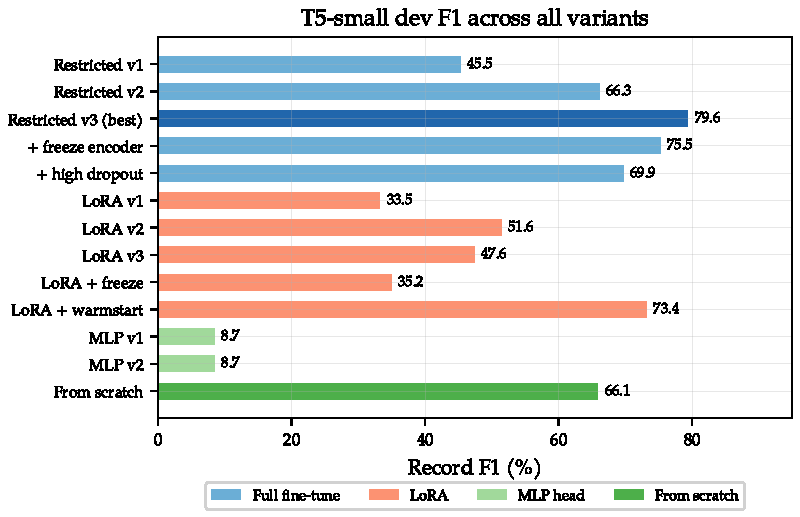
\includegraphics[width=0.92\linewidth]{../media/dev_f1_comparison.pdf}
    \end{center}
  }

  \block{Approach 2: Training From Scratch}{
    \begin{itemize}[nosep, leftmargin=*]
      \item Same T5-small architecture from \textbf{random initialization}
      \item Required 8 hours and 98 epochs (vs.\ 75 min for fine-tuning)
      \item Reached 66.1\% F1 -- \textbf{13.5pp below} the fine-tuned model
      \item Demonstrates the value of pretrained representations
    \end{itemize}
  }

  \block{Approach 3: DPO Post-Training}{
    \begin{itemize}[nosep, leftmargin=*]
      \item \textbf{Direct Preference Optimization} on top of best SFT model (T5-base, F1=86.0\%)
      \item 9,801 preference triplets: model-generated negatives + execution-aware perturbations
      \item Loss: $\mathcal{L}_\text{DPO} = -\log\sigma\bigl(\beta[\Delta\log\pi_\theta - \Delta\log\pi_\text{ref}]\bigr)$
      \item Swept $\beta$, LR, full fine-tune vs.\ LoRA
      \item \textbf{Did not improve}: restricted vocab already constrains output space; reward hacking observed (margin grew $1.6 \to 12.2$ while F1 collapsed)
    \end{itemize}
  }

  % ══════════════════════════════════════════════════════════
  % RIGHT COLUMN
  % ══════════════════════════════════════════════════════════
  \column{0.33}

  \block{Results}{
    \begin{center}
    \large
    \begin{tabular}{lccc}
      \toprule
      \textbf{System} & \textbf{SQL EM} & \textbf{Rec.\ EM} & \textbf{Rec.\ F1} \\
      \midrule
      \multicolumn{4}{l}{\emph{Dev Results}} \\
      \midrule
      T5-small SFT (best)    & 58.80 & --   & 79.60 \\
      T5-small from scratch  & 50.43 & --   & 66.12 \\
      T5-base SFT (best)     & 73.39 & 84.76 & \textbf{85.96} \\
      DPO on T5-base         & 71.24 & 83.69 & 84.82 \\
      \midrule
      \multicolumn{4}{l}{\emph{Test Results}} \\
      \midrule
      T5-small SFT           & 0.00  & --   & 55.25 \\
      T5-small from scratch  & 0.00  & --   & 59.16 \\
      \bottomrule
    \end{tabular}
    \end{center}

    \begin{center}
      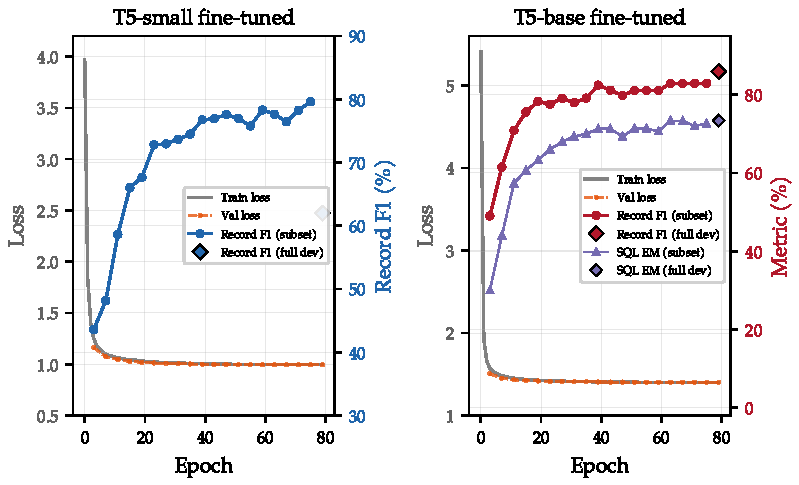
\includegraphics[width=0.92\linewidth]{../media/training_curves.pdf}
    \end{center}
  }

  \block{Key Findings}{
    \begin{enumerate}[nosep, leftmargin=*]
      \item \textbf{Pretraining matters}: 79.6\% vs.\ 66.1\% F1 (+13.5pp) -- pretrained representations provide strong initialization for NL-to-SQL
      \item \textbf{Scale helps}: T5-base (222M) reaches 86.0\% F1 vs.\ T5-small (60M) at 79.6\% (+6.4pp)
      \item \textbf{Schema augmentation is critical}: +13.7pp F1 from adding table names to encoder input
      \item \textbf{DPO hits a ceiling}: restricted decoder vocab (598 tokens) leaves little room for preference optimization
    \end{enumerate}
  }

  \block{References}{
    {\small
    [1] Rafailov et al.\ \textit{Direct Preference Optimization}. NeurIPS 2023. \\[2pt]
    [2] Raffel et al.\ \textit{Exploring the Limits of Transfer Learning with T5}. JMLR 2020. \\[2pt]
    [3] Hu et al.\ \textit{LoRA: Low-Rank Adaptation of LLMs}. ICLR 2022.
    }
  }

\end{columns}
\end{document}
